

\tikzset{every picture/.style={line width=0.75pt}} %set default line width to 0.75pt        

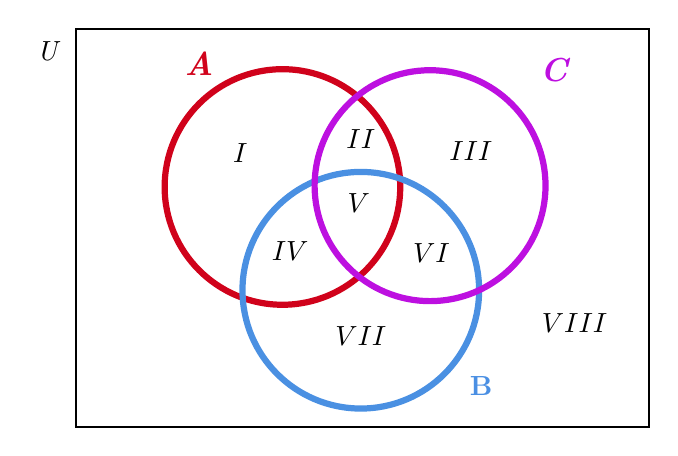
\begin{tikzpicture}[x=0.75pt,y=0.75pt,yscale=-1,xscale=1]
%uncomment if require: \path (0,222); %set diagram left start at 0, and has height of 222

%Shape: Circle [id:dp6019981075283429] 
\draw  [color={rgb, 255:red, 208; green, 2; blue, 27 }  ,draw opacity=1 ][line width=2.25]  (209.5,87.25) .. controls (209.5,55.91) and (234.91,30.5) .. (266.25,30.5) .. controls (297.59,30.5) and (323,55.91) .. (323,87.25) .. controls (323,118.59) and (297.59,144) .. (266.25,144) .. controls (234.91,144) and (209.5,118.59) .. (209.5,87.25) -- cycle ;
%Shape: Circle [id:dp707293905477145] 
\draw  [color={rgb, 255:red, 74; green, 144; blue, 226 }  ,draw opacity=1 ][line width=2.25]  (247,137) .. controls (247,105.52) and (272.52,80) .. (304,80) .. controls (335.48,80) and (361,105.52) .. (361,137) .. controls (361,168.48) and (335.48,194) .. (304,194) .. controls (272.52,194) and (247,168.48) .. (247,137) -- cycle ;
%Shape: Circle [id:dp13160094529110977] 
\draw  [color={rgb, 255:red, 189; green, 16; blue, 224 }  ,draw opacity=1 ][line width=2.25]  (281.75,86.63) .. controls (281.75,55.9) and (306.65,31) .. (337.38,31) .. controls (368.1,31) and (393,55.9) .. (393,86.63) .. controls (393,117.35) and (368.1,142.25) .. (337.38,142.25) .. controls (306.65,142.25) and (281.75,117.35) .. (281.75,86.63) -- cycle ;
%Shape: Rectangle [id:dp3258541513105915] 
\draw   (167,11) -- (443,11) -- (443,203) -- (167,203) -- cycle ;

% Text Node
\draw (397,31) node [scale=1,color={rgb, 255:red, 80; green, 227; blue, 194 }  ,opacity=1 ] [align=left] {{\large \textbf{\textit{\textcolor[rgb]{0.74,0.06,0.88}{C}}}}};
% Text Node
\draw (362,183) node [scale=1,color={rgb, 255:red, 80; green, 227; blue, 194 }  ,opacity=1 ] [align=left] {\textcolor[rgb]{0.29,0.56,0.89}{\textbf{B}}};
% Text Node
\draw (226,28) node [scale=1,color={rgb, 255:red, 245; green, 166; blue, 35 }  ,opacity=1 ] [align=left] {\textit{\textcolor[rgb]{0.82,0.01,0.11}{{\large \textbf{A}}}}};
% Text Node
\draw (246,71) node   {$I$};
% Text Node
\draw (304,64) node   {$II$};
% Text Node
\draw (357,70) node   {$III$};
% Text Node
\draw (303,95) node   {$V$};
% Text Node
\draw (270,118) node   {$IV$};
% Text Node
\draw (338,119) node   {$VI$};
% Text Node
\draw (304,159) node   {$VII$};
% Text Node
\draw (407,153) node   {$VIII$};
% Text Node
\draw (154,22) node  [align=left] {\textit{U}};


\end{tikzpicture}